\begin{problem}{멀티드링크}
	{standard input}{standard output}
	{1 seconds}{128 megabytes}{}
	
	
	Byteasar는 구석구석에 있는 ``우유 바"로 유명한 도시인 Byteburg에 산다. 어느날, Byteasar는 ``우유 멀티드링크"라는 아이디어를 떠올려 냈다: 그는 모든 우유 바에 정확히 한 번 방문하여 우유를 마시고 싶어 한다. 이상적으로, Byteasar는 이전 우유 바와 다음 우유 바 사이가 두 블럭(교차로)을 넘지 않게 경로를 만들고 싶다.
	
	Byteburg의 교차로는 1부터 $n$까지 번호가 붙어있고, 모든 도로는 양방향이다. Byteburg의 모든 두 교차로 쌍에는 같은 교차로를 두 번 이상 방문하지 않는 단순 경로가 정확히 하나 존재한다. Byteasar의 경로는 1번 교차로에서 시작하고, $n$번 교차로에서 끝난다.
	
	당신이 할 일은 Byteasar의 조건을 만족하는 경로를 아무거나 하나 찾는 것이다.
	
	\begin{center}
	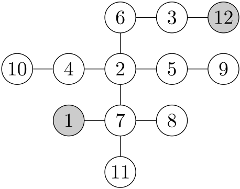
\includegraphics[width=0.3\linewidth]{mul1.png}
	\end{center}
	
	조건을 만족하는 경로중 하나는: 1, 11, 8, 7, 5, 9, 2, 10, 4, 6, 3, 12이다.
	
	\begin{center}
		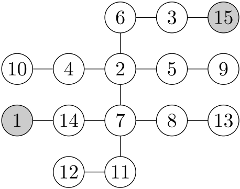
\includegraphics[width=0.3\linewidth]{mul2.png}
	\end{center}
	 
	이 경우에는 조건을 만족하는 경로가 없다.
	

	\InputFile
	
	첫째 줄에는, Byteburg의 교차로의 수를 나타내는 $n$이 들어온다.($2 \le n \le 500,000$) 
	
	다음 $n-1$개의 줄 각각에는 서로 다른 두 정수 $a_i$와 $b_i$가 공백 하나로 구분되어 들어온다. 이는 교차로 $a_i$와 $b_i$사이에 도로가 있다는 의미이다.
	
	\OutputFile
	
	만약 Byteasar의 조건을 만족하는 경로가 없다면 ``\texttt{BRAK}"을 출력한다.  (따옴표는 출력하지 않는다.) 경로가 존재 한다면 $n$개의 줄을 출력하는데, $i$번째에는 Byteasar의 조건을 만족하는 경로의 $i$번째 교차로의 번호를 출력하여야 한다. 당연하게도 첫째 줄에는 1을, $n$번째 줄에는 $n$을 출력해야 한다.
	
	 
	\Examples
		
	\begin{example}
	\exmp{
	12
	1 7
	7 8
	7 11
	7 2
	2 4
	4 10
	2 5
	5 9
	2 6
	3 6
	3 12
	}{%
	1
	11
	8
	7
	4
	10
	2
	9
	5
	6
	3
	12 
	}%
	\exmp{
	15
	1 14
	14 7
	7 8
	7 11
	7 2
	2 4
	4 10
	2 5
	5 9
	2 6
	3 6
	3 15
	11 12
	8 13
	}{%
	BRAK
	}%
	\end{example}
        
\end{problem}

